To get some more insight in to the behaviour of the indexing techniques that we applied, we performed further analysis of the data. This gave us some further useful explanations. We wanted to ascertain that a typical fingerprint dataset is high dimensional and highly sparse almost follwing a power law sort of distribution with very few features occuring in almost all the points in the chemical database while majority of the features have a non-zero value in very few points. We wanted to extract patterns in the data which could be exploited for range search querying and point querying.\\

\section{A Typical Fingerprint Dataset Analysis}
We performed a detailed analysis of the data to figure out the kind of indexing technique, which needs to be used to optimize our searching time. The statistics that were extracted from the data are as follows:\\

\begin{table}[ht!]
\centering
\caption{Statistics of Data}
\begin{tabular}{|l|c|}
\hline 
Number of data points & 264016 \\ 
Number of unique features is & 785985 \\ 
Maximum number of features in a data point is & 1903 \\ 
Minimum number of features in a data point is  & 7 \\ 
Average number of features in a data point is & 270.602966 \\ 
Maximum number of data point with a feature is & 259110 \\ 
Minimum number of data point with a feature is & 1 \\ 
Average number of data point with a feature is & 90
 \\ 
Maximum value of a feature  & 1870 \\ 
Minimum value of a feature
 & 1 \\ 
Average value of a feature & 1.142210 \\ 
Maximum number of heavy-hitters  & 144 \\ 
Minimum number of heavy-hitters  & 1 \\ 
 Average number of heavy-hitters  & 44.5 \\ 
\hline 
\end{tabular} 
\end{table}

From this we can observe that the data is highly sparse with only about 271 features, on a average, in a point, as opposed to the 785985 unique features. This high sparsity makes the data set an ideal candidate to perform inverted indexing. In inverted indexing, instead of indexing the data points we would index the features. This leads to a large index structure, but we gain on the speed of point query. \\

\begin{figure}[ht!]	
\centering
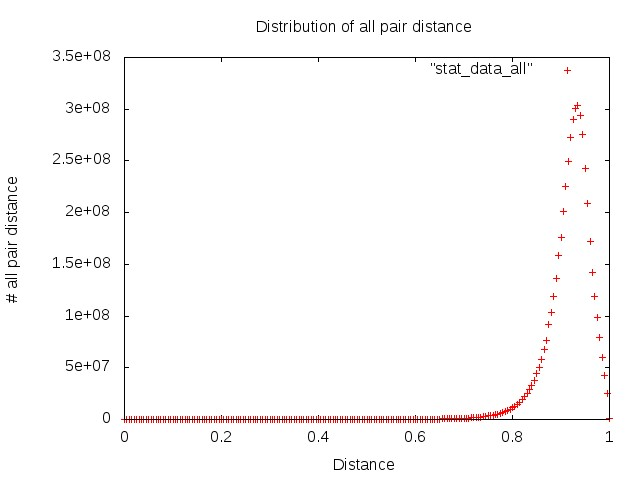
\includegraphics[width=0.7 \columnwidth]{img/all.jpg}
\caption{All pair distances}
\end{figure}
%\pagebreak
\begin{figure}[ht!]	
\centering
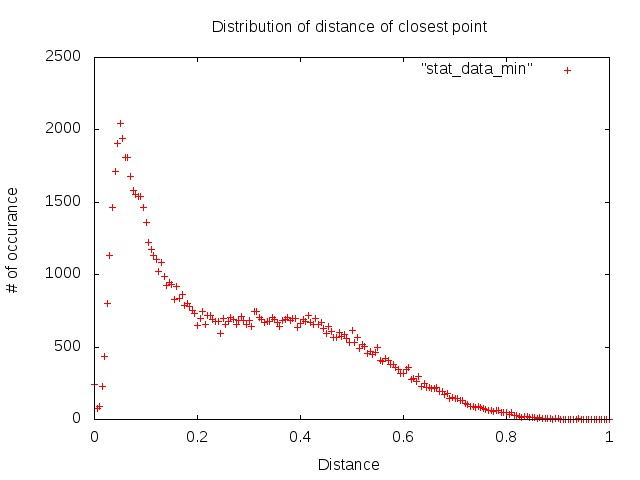
\includegraphics[width=0.7 \columnwidth]{img/min.jpg}
\caption{Distance of the closest point}
\end{figure}

\begin{figure}[ht!]	
\centering
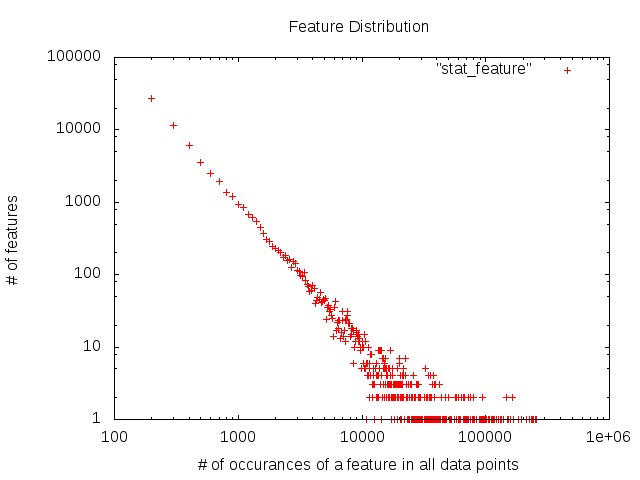
\includegraphics[width=0.7 \columnwidth]{img/feature.jpg}
\caption{Feature distribution}
\end{figure}


\section{Observations on the Data}

What we can observe from the data are the following:
\begin{enumerate}

\item {The being in high dimension, is very much spread out, and hence most of the points are equidistant from each other.}\\

\item {The closest point for most of the points is at distance much greater than 0.4. in fact only 0.007\% of the points have their 1-NN within a distance of 0.4.}\\

\item {the distribution of features among the data points seem to follow a power law distribution (though we have not tried to regress the plot to a function) i.e., even though we have many features only a hand full of them are repeated in most of the points.}\\

\item {One of the most time consuming operations in our algorithms has been the recurring theme of finding the set of maximally separated points, which we called as pivots. It takes hours for the algorithm to converge. Given the distribution of all pairs distance, we cannot hope to improve it further, but we can propose an heuristic streaming algorithm to handle it efficiently.\\ \\
	We can maintain a list of most frequently occurring farthest points. These points are not necessarily the points farthest from each other, but the points which are most frequent in the list farthest points, for each point. This is motivated from the frequency counting problem from streaming as shown in \citet*{metwally2005efficient}.}\\

\item  {We observed that the inverted index we proposed could not be easily generalised  to range queries. This can be further observed from the fact that how skewed the data distribution is.\\ \\
	Given that only 0.007\% of the 1-nn points have distance less that 0.4, we can never achieve a efficient pruning. And in addition the distribution of heavy-hitters (features with occurrence more that 50000) is also very high, We have on an average 44 heavy hitters in a data point. Hence, in the worst case, we will be forced to explore all the points.} \\

\item  {The success of any embedding technique, especially Lipschitz, depends on the ability of the reference set to be representative of the entire data. in our case, given that the entire data is very widely spread, the number of reference set required to well represent the data, becomes very large. This is the reason why Lipschitz did not give the desired results.}
\end{enumerate}
